\PassOptionsToPackage{rgb}{xcolor}
\documentclass[tikz,border=10pt]{standalone}
\usetikzlibrary{mindmap}
\begin{document}
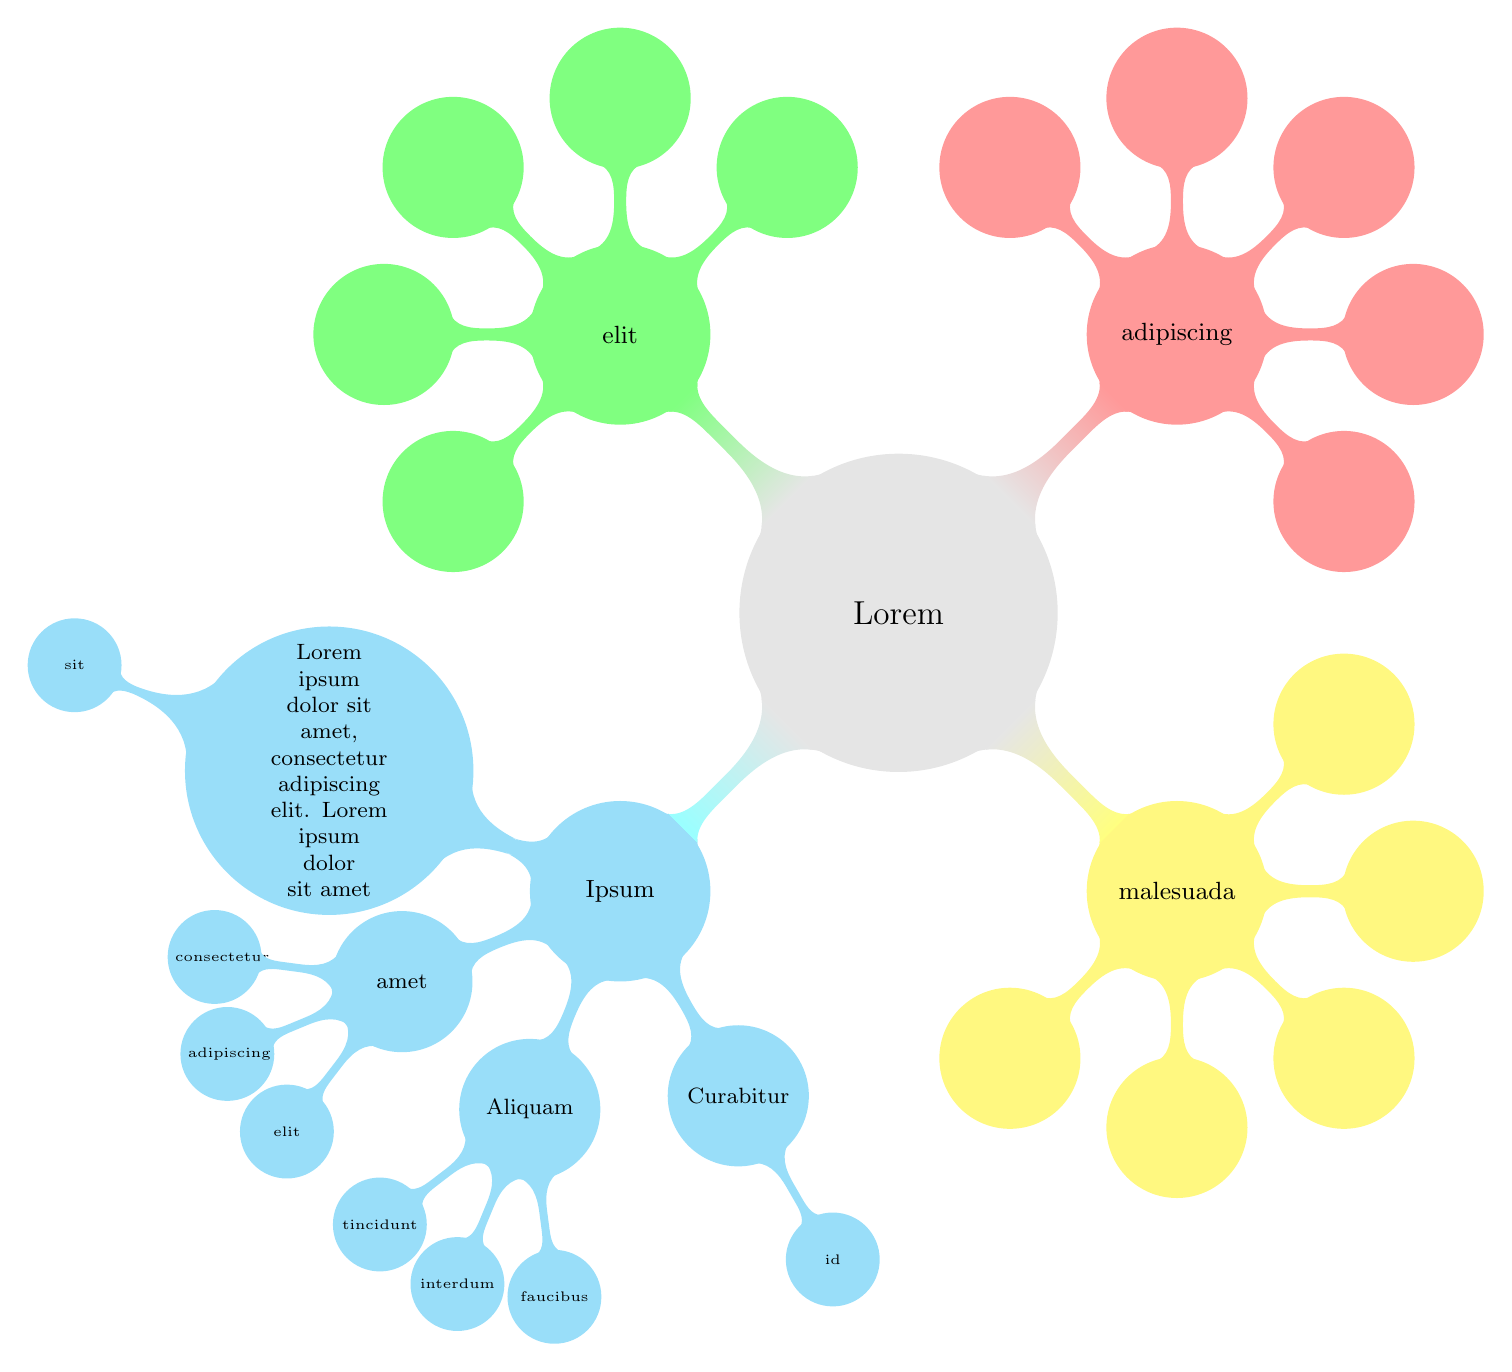
\begin{tikzpicture}
  \path
  [
    mindmap,
    grow cyclic,
    every node/.style=concept,
    concept color=black!10,
    level 1/.append style={level distance=5cm, sibling angle=90},
    level 2/.append style={level distance=3cm, sibling angle=45},
    root concept/.append style={concept, concept color=black!10},
  ]
  node [root concept] {Lorem}
   child [concept color=cyan!40] { node {Ipsum}
        child [level distance=40mm] { node {Lorem ipsum dolor sit amet, consectetur adipiscing elit. Lorem ipsum dolor sit amet}
            child [level distance=35mm] { node {sit}}
               }
        child { node {amet}
            child { node {consectetur}}
            child { node {adipiscing}}
            child { node {elit}}
        }
        child { node {Aliquam}
            child { node {tincidunt}}
            child { node {interdum}}
            child { node {faucibus}}
               }
        child [style={sibling angle=50}] { node {Curabitur}
            child{ node {id}}
               }
    }
    child [concept color=yellow!50] { node {malesuada}
        child { node {}}
        child { node {}}
        child { node {}}
        child { node {}}
        child { node {}}
    }
    child [concept color=red!40] { node {adipiscing}
        child { node {}}
        child { node {}}
        child { node {}}
        child { node {}}
        child { node {}}
    }
    child [concept color=green!50] { node {elit}
        child { node {}}
        child { node {}}
        child { node {}}
        child { node {}}
        child { node {}}
    };
\end{tikzpicture}
\end{document}